\documentclass{article}
\title{\Large  Physics 21 - – Strings and Webs}
\author{\large Shubh Agrawal, \normalsize\emph{Class of 2022}}
\date{\small July 16, 2019}
\usepackage[a4paper,top=1cm, left=1cm,width=1cm,bottom=1cm,right=1cm]{geometry}
\usepackage{amsthm, amsmath, amssymb, tipa, graphicx, caption, subcaption, float}
\usepackage{geometry}
\usepackage{listings}
\usepackage{color}
\usepackage[usenames,dvipsnames,svgnames,table]{xcolor}

\begin{document}

\maketitle
\subsection*{Introduction}
We attempt to obtain time-dependent intensity data for the variable system Her X-1 from the Catalina (CTRS) Surveys. Two methods were used, which are described under the two separate sections below. The first involves scarping the webpage in \textit{.html} format and using string manipulations to generate two lists and plot them. The second involves downloading the data in \textit{VOTable} format, and attempting to obtain the same plot as under (taken from the CRTS website). Source code is available in the file \textit{lab1.py}, while the VOTable \textit{.xml} file is attached as Appendix at the end of this document.
\begin{figure}[H]
	\centering
	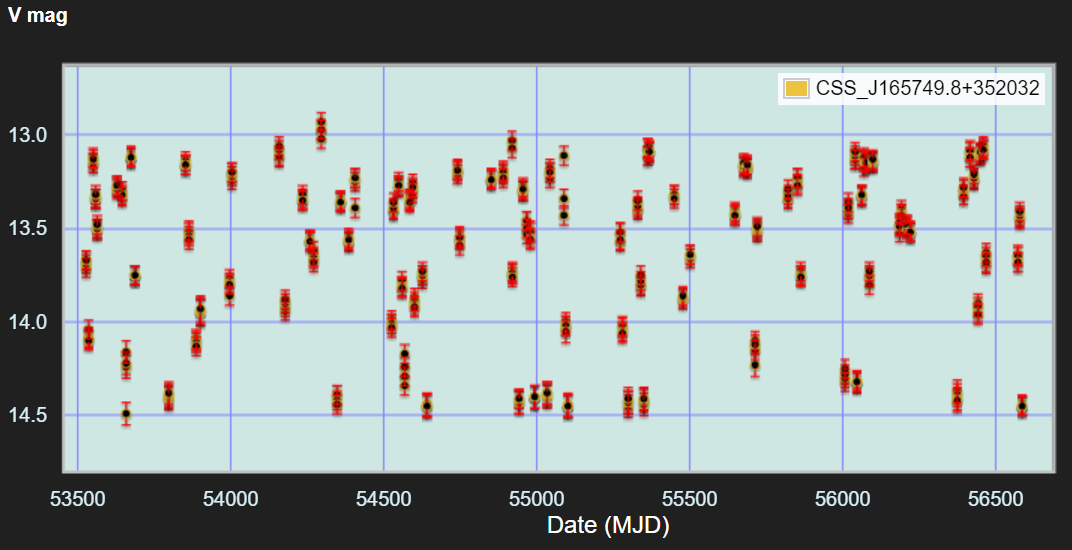
\includegraphics[width = 0.8\textwidth]{org.png}
	\label{orig}
	\caption{Original magnitude versus time (in mean Julian days) plot.}
\end{figure}
\pagebreak
\subsection*{Part 1: HTML format}
HTML data for the system Her X-1, from the photcal survey in short form, was obtained from \textit{http://nesssi.cacr.caltech.edu/cgi-bin/getcssconedbid\_release2.cgi}. The file was decoded to text, and string manipulations were used to get the below plot.
\begin{figure}[H]
	\centering
	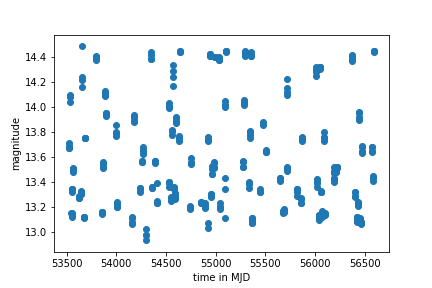
\includegraphics[width = 0.8\textwidth]{html.png}
	\label{html}
	\caption{Magnitude versus Time (in mean Julian days) plot, obtained using the \textit{getValues()} function.}
\end{figure}

\subsection*{Part 2: VOTable format}
VOTable data for the system Her X-1, from the photcal survey in short form, was obtained from \textit{http://nesssi.cacr.caltech.edu/DataRelease/upload/result\_web\_fileyUkAfF.vot}. The file was saved as .xml, and array manipulations were used to get the below plot.
\begin{figure}[H]
	\centering
	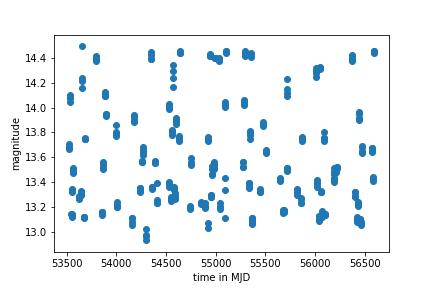
\includegraphics[width = 0.8\textwidth]{vot.png}
	\label{vot}
	\caption{Magnitude versus Time (in mean Julian days) plot, obtained using the \textit{getVOTvalues()} function.}
\end{figure}
\subsection*{Result}
The two graphs obtained from the scarped data are similar to the plot given on the CRTS site.
\subsection*{Appendix}
\lstset{
	language=xml,
	tabsize=3,
	%frame=lines,
	caption = VOTable file (in .xml format) obtained and used.,
	label=code:sample,
	frame=shadowbox,
	rulesepcolor=\color{gray},
	xleftmargin=20pt,
	framexleftmargin=15pt,
	keywordstyle=\color{blue}\bf,
	commentstyle=\color{OliveGreen},
	stringstyle=\color{red},
	numbers=left,
	numberstyle=\tiny,
	numbersep=5pt,
	breaklines=true,
	showstringspaces=false,
	basicstyle=\footnotesize,
	emph={food,name,price},emphstyle={\color{magenta}}}
\lstinputlisting{data.xml}

\end{document}